\subsection{Advanced R Profiling}
\makesubcontentsslidessec

\begin{frame}
  \begin{block}{Other Profiling Tools}
    \begin{itemize}
      \item perf
      \item PAPI
      \item MPI profiling: fpmpi, mpiP, TAU
    \end{itemize}
  \end{block}
\end{frame}



\begin{frame}[fragile]
  \begin{block}{Profiling MPI Codes with \textbf{pbdPROF}}
  \begin{minipage}[t]{.58\textwidth}
  \vspace{.2cm}
  \vspace{0pt}
  1. Rebuild \pbdR\ packages
\vspace*{-.5cm}
\begin{lstlisting}[language=shl,title=\ ]
R CMD INSTALL pbdMPI_0.2-1.tar.gz \ --configure-args= \ "--enable-pbdPROF"
\end{lstlisting}
2. Run code
\vspace*{-.5cm}
\begin{lstlisting}[language=shl,title=\ ]
mpirun -np 64 Rscript my_script.R
\end{lstlisting}

3. Analyze results
\vspace{-.5cm}
\begin{lstlisting}[title=\ ]
library(pbdPROF)
prof <- read.prof( "output.mpiP")
plot(prof, plot.type="messages2")
\end{lstlisting}

  \end{minipage}
  \hfill
  \begin{minipage}[t]{.4\textwidth}
  \vspace{0pt}
    \centering
    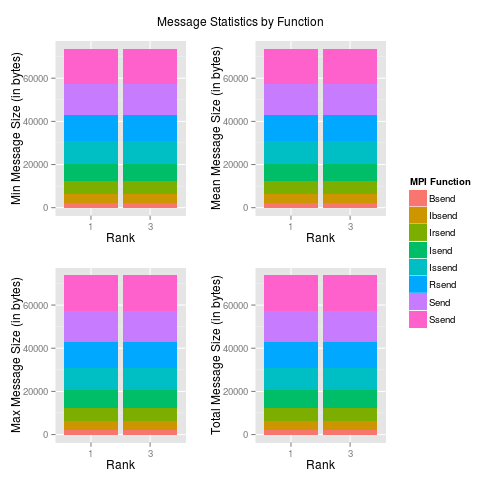
\includegraphics[scale=.25]{../common/pics/mpip}
    \\[.1cm]
    
\includegraphics[scale=0.35]{../common/pics/gsoc}
  \end{minipage}
  \end{block}
\end{frame}



\begin{frame}[fragile]
  \begin{block}{Profiling with \textbf{pbdPAPI}}
  \begin{minipage}{.6\textwidth}
    \begin{itemize}
      \item Bindings for Performance Application Programming Interface (PAPI)
      \item Gathers detailed hardware counter data.
      \item High and low level interfaces
    \end{itemize}  
  \end{minipage}
  \begin{minipage}{.38\textwidth}
    \centering
    
\includegraphics[scale=0.12]{../common/pics/gsoc_2014}
  \end{minipage}
\begin{center}
\begin{tabular}{ll} \hline\hline
Function & Description of Measurement \\ \hline
\code{system.flips()} & Time, floating point instructions, and Mflips \\
\code{system.flops()} & Time, floating point operations, and Mflops \\
\code{system.cache()} & Cache misses, hits, accesses, and reads \\
\code{system.epc()} & Events per cycle \\
\code{system.idle()} & Idle cycles \\
\code{system.cpuormem()} & CPU or RAM bound$^*$ \\
\code{system.utilization()} & CPU utilization$^*$ \\
\hline\hline
\end{tabular}
\end{center}
  \end{block}
\end{frame}
